\addtocontents{toc}{\protect\newpage}
\chapter{Appendix 1}
\section{Codesnippet 1}
	\lstinputlisting[language=C++,caption=Totaalverzicht van de YUV-RGB conversie en frame-iteratie, label = app:codesnippet1]{Chapters/Chapter2/SourceCode/RGBtoYUVcomplete.c}

\newpage
\section{Codesnippet 2}
\lstinputlisting[language=C++,caption=Kleurenconversie met enkele iteratie, label=lis:video_A.c]{Chapters/Chapter2/SourceCode/video_A.c}

\newpage
\section{Codesnippet 3}
\lstinputlisting[language=C++,caption=Aanpassingen aan de linker file voor 32-dubbele buffering, label=lis:video_in_out.ldf, firstline=374, lastline=405]{Chapters/Chapter2/SourceCode/video_in_out.ldf}

\newpage
\section{Codesnippet 4}
\lstinputlisting[language=C++,caption=Aanpassingen aan system.h voor 32-dubbele buffering, label=lis:system.h]{Chapters/Chapter2/SourceCode/system.h}

\newpage
\section{Codesnippet 5}
\lstinputlisting[language=C++,caption=Aanpassingen aan L3\textunderscore SDRAM.h voor 32-dubbele buffering, label=lis:L3_SDRAM.h]{Chapters/Chapter2/SourceCode/L3_SDRAM.h}

\newpage
\section{Codesnippet 6}
\lstinputlisting[language=C++,caption=Aanpassingen aan L3\textunderscore SDRAM.c voor 32-dubbele buffering, label=lis:L3_SDRAM.c]{Chapters/Chapter2/SourceCode/L3_SDRAM.c}

\newpage
\section{Codesnippet 7}
\lstinputlisting[language=C++,caption=Kleurenconversie met pixel skipping, label=lis:video_A_block.c]{Chapters/Chapter2/SourceCode/video_A_block.c}

\chapter{Appendix 2}
\newpage
\section{Algemeen overzicht}
\label{app:algemeenoverzicht}
	\begin{figure}[H]
		\centering
		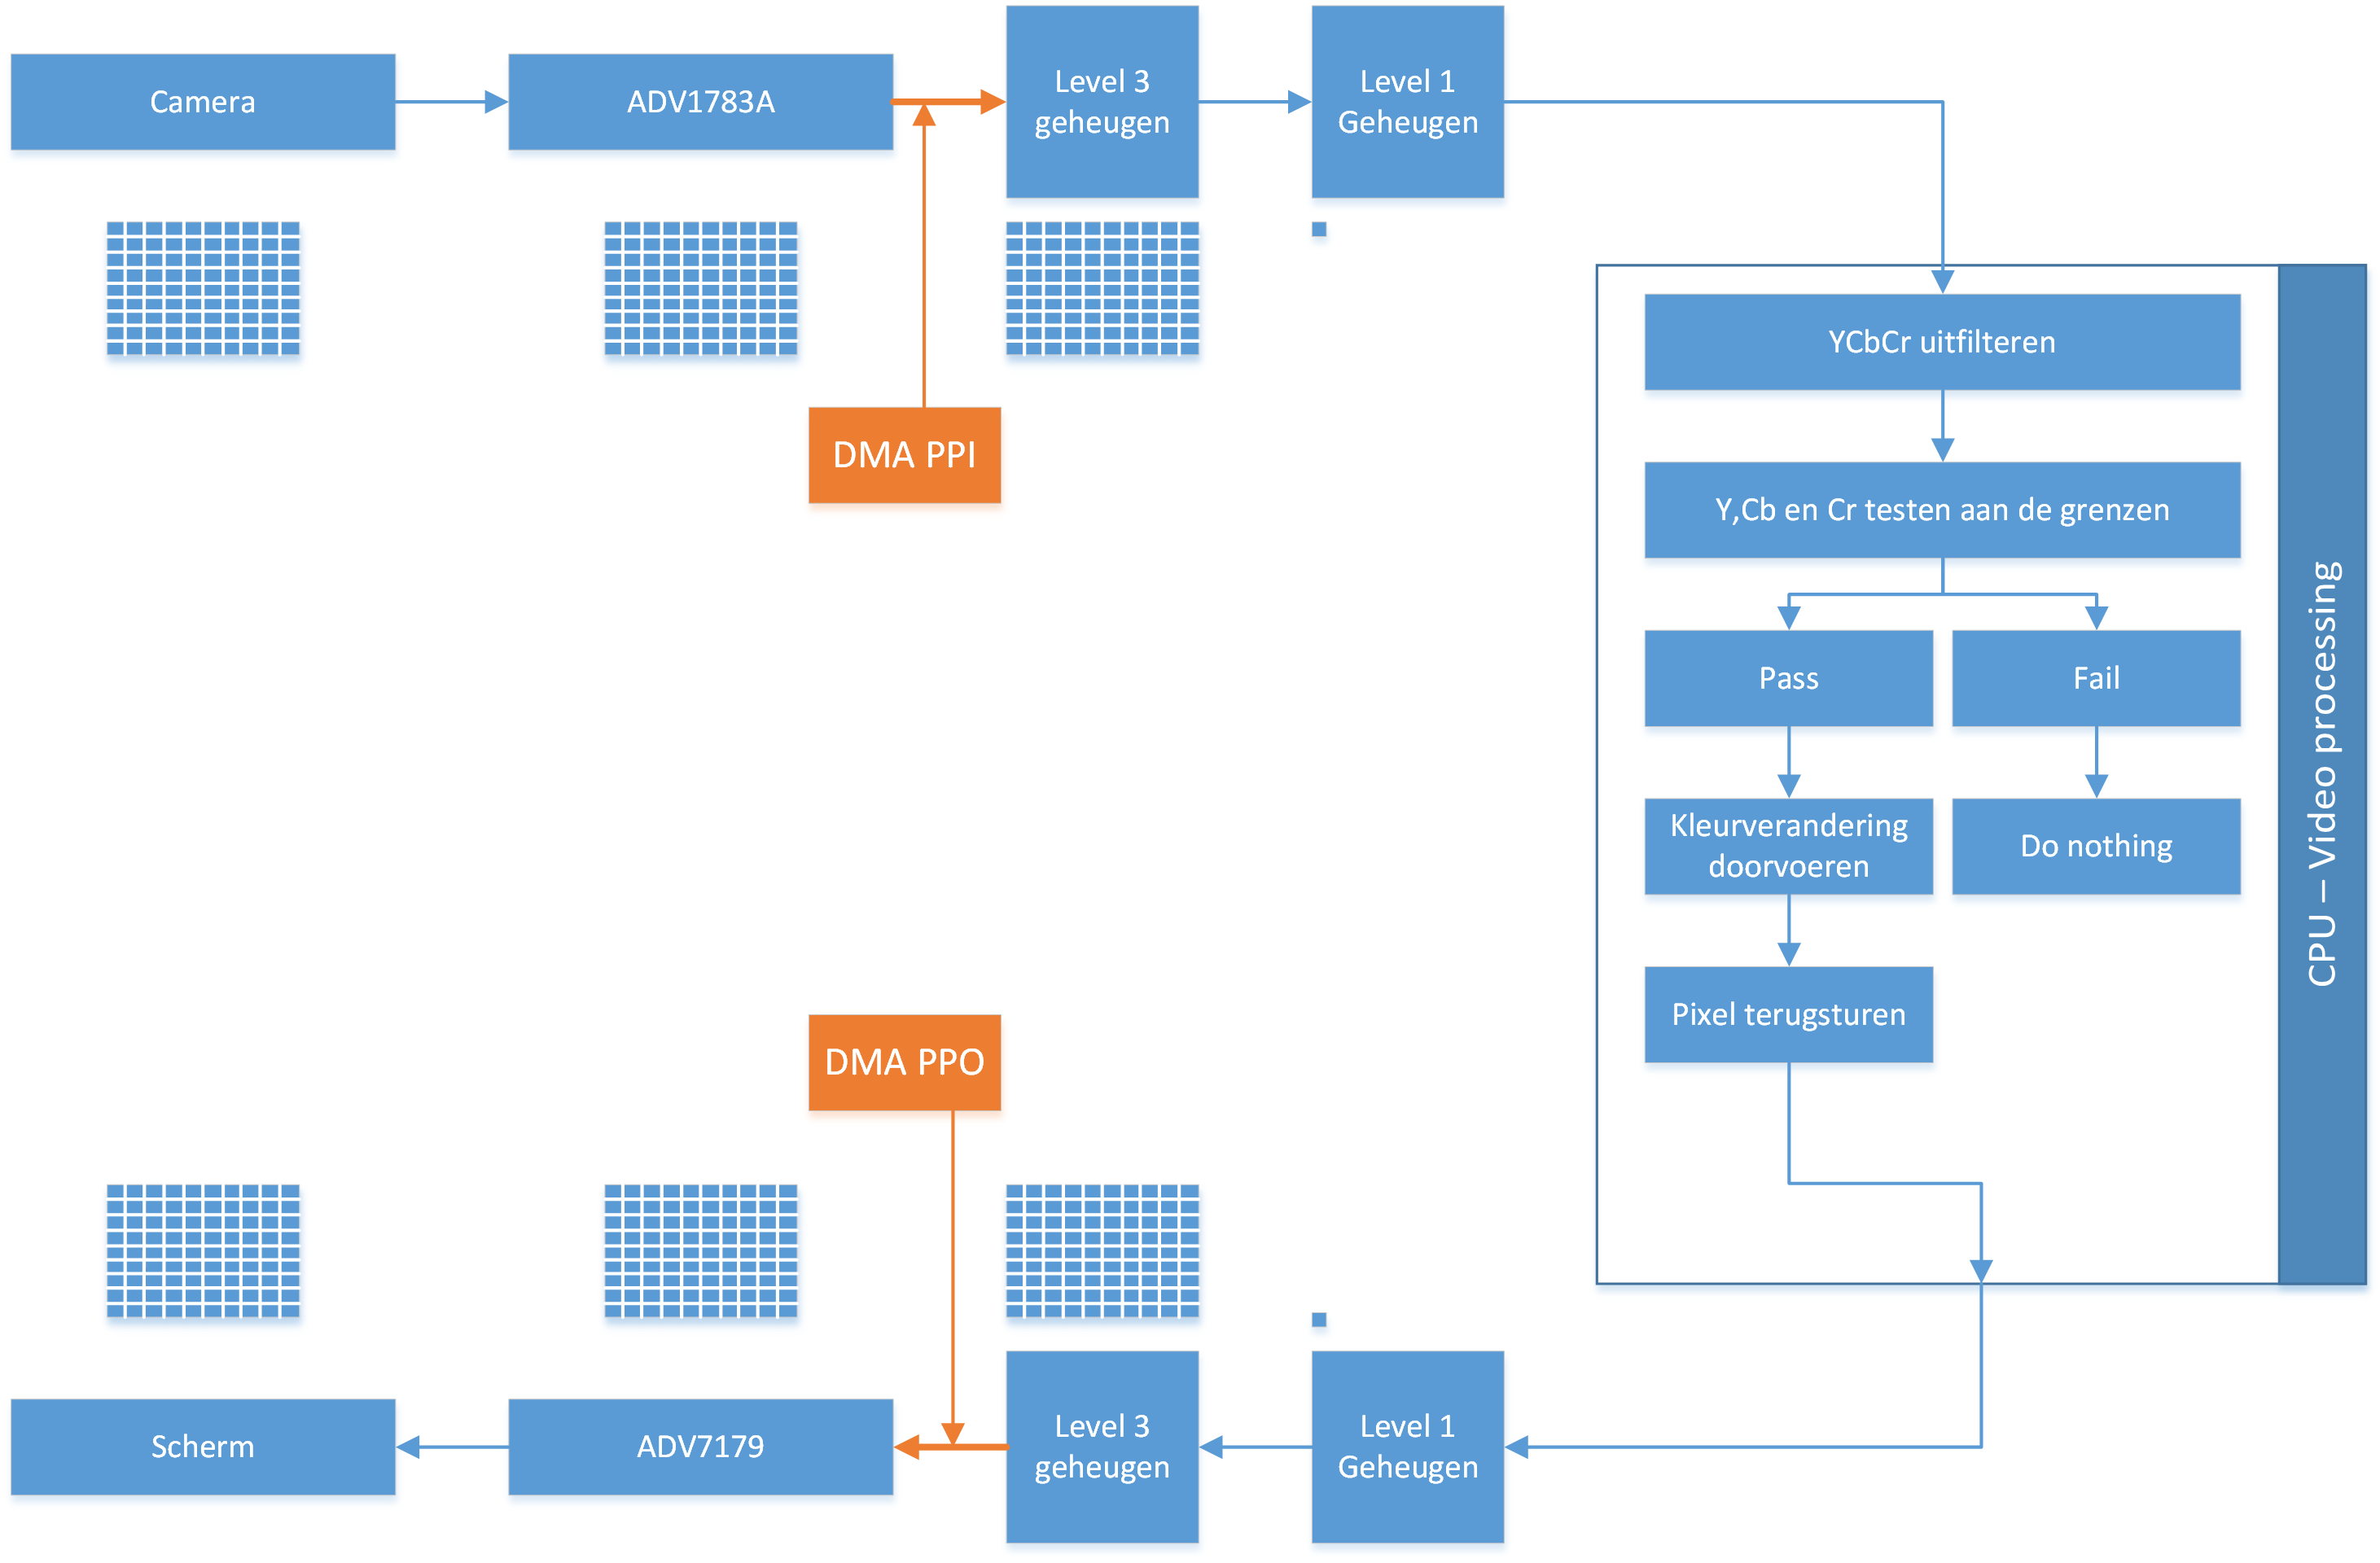
\includegraphics[width=19cm, angle = 90]{Chapters/Chapter2/Images/implementationOverview.png}
		\caption{Algemeen overzicht van de implementatie op de BlackFin BF-561}
	\end{figure}